\chapter{He Turned \$100k Into \$25M}

This chapter follows Todd Napola's interview as a source-conscious case study in commercial real estate judgment. The mathematics is not blackboard mathematics; it is the arithmetic of a deal: cash committed, value created, debt placed, capital returned, and cash flow retained. We will keep the spoken order of the interview: first the promise, then mentorship, then the first property, then the question of capital, operating edge, scale, and finally the reason a business can be rebuilt after money itself disappears.

\section{The Promise: From Zero Cash to an Eight-Figure Portfolio}

The interview opens with the outcome before it gives us the mechanism. Todd Napola is introduced as a Miami commercial real estate operator who, over roughly twenty-five years, built an eight-figure real estate portfolio. The origin story is sharper than the outcome: at twenty-five years old, he drained his bank account to buy his first property.

That ordering matters. The lecture does not begin with a theory of real estate. It begins with a risk: money going almost to zero in exchange for control of an asset. Later, that same pattern reappears at larger scale in a \$25 million shopping-center acquisition. The first property is the small model; the later deal is the scaled version.

The host also previews a rule that will return later: if an extraordinary deal is available, capital is less scarce than the deal itself. We should not take that as a universal theorem. We should read it as Todd's claim about commercial real estate markets: investors line up for genuinely good deals, while truly good deals are hard to find.

\section{Mentorship as an Acquisition of Judgment}

The first direct question is simple: what advice would Todd give to a new entrepreneur? His answer is not a formula or a market indicator. It is ``find a mentor,'' and he says he would repeat it many times.

The story that follows is the real instruction. Todd hears Gary Rappaport speak at a real estate convention. Rappaport leaves business cards around the room and says that people will take them, but almost nobody will call. Todd notices the challenge inside that statement. He does not merely take the card; he waits outside the booth, introduces himself, and asks to visit the office of someone doing the work he wants to do.

The sequence is important:
\begin{enumerate}
\item He identifies a person whose business matches his own ambition.
\item He takes the public offer of help literally.
\item He changes the offer from vague advice into a concrete visit.
\item He pays the travel cost and shows up.
\item He turns one meeting into an ongoing relationship.
\end{enumerate}

Later, when Todd tells Gary about closing a \$25 million deal, Gary answers by mentioning a \$125 million deal and tells him, in effect, to keep going. The point is not humiliation. The point is scale calibration: a mentor changes the size of what seems normal.

\subsection{Question \& Answer}

\paragraph{Question.}
If successful people are willing to help, why does asking for help so often fail?

\paragraph{Answer.}
Because the offer of help is usually left in a vague state. Todd's story turns help into action. A business card becomes a meeting; a meeting becomes a flight; a flight becomes a day in the mentor's office; the office visit becomes a durable relationship. The mechanism is not ``having access'' in the abstract. It is converting access into repeated contact with someone whose judgment is already formed in the field one wants to enter.

\section{The First Property: Risk, Repair, Refinance, Cash Flow}

After the mentorship story, the interview moves through a financial-advice passage: do not count other people's money. Todd connects this to social comparison, appearances, cars, dinners, and social media. The advice is defensive. It clears away the false scoreboard before the real risk story begins.

The central numerical sequence starts when Todd explains why he wanted real estate. He was a stockbroker in the 1990s and doing well, but commission income had a hard limitation: if there was no trade, there was no money. Even a vacation meant no commission for that week. Real estate appears here as an answer to labor-tied income.

Todd says that at twenty-five he bought his first property and drained a six-figure bank account down to \$50. He then gives the numbers of the deal:
\begin{equation}
P_{\mathrm{buy}}=\$575{,}000,\qquad C_{\mathrm{remaining}}=\$50.
\end{equation}

The property was not left alone. Todd says he re-tenanted it, cleaned it up, used friends as cheap labor, painted it, improved how it looked, and wrote leases for new tenants. That operating work is the hinge between purchase and refinance.

He then says that in December of that year he refinanced the property at an \$800,000 value and obtained a \$600,000 loan. The transcript wording is imperfect, so we treat \$800,000 cautiously as the refinance valuation:
\begin{equation}
V_{\mathrm{refi}}=\$800{,}000,\qquad L_{\mathrm{refi}}=\$600{,}000.
\end{equation}

The standard arithmetic attached to those two numbers is the loan-to-value ratio:
\begin{equation}
\mathrm{LTV}
=
\frac{L_{\mathrm{refi}}}{V_{\mathrm{refi}}}
=
\frac{600{,}000}{800{,}000}
=
0.75
=
75\%.
\end{equation}

This is not a phrase Todd uses in the interview. It is our clean reconstruction of the financing arithmetic from his stated numbers.

\begin{table}
\centering
\begin{tabular}{ll}
\hline
Quantity & Amount or value \\
\hline
First property purchase price & \$575,000 \\
Cash left after purchase & \$50 \\
Refinance value, stated cautiously & \$800,000 \\
Refinance loan & \$600,000 \\
Inferred loan-to-value & 75\% \\
Monthly free cash flow & \$5,000 \\
Annualized free cash flow & \$60,000 \\
\hline
\end{tabular}
\caption{Transcript-backed numbers from Todd Napola's first-property story, with simple arithmetic reconstructions marked in the surrounding text.}
\end{table}

Todd says the refinance returned all his money and closing costs, while leaving him with \$5,000 per month in free cash flow beginning the following January. Annualized, that cash flow is
\begin{equation}
CF_{\mathrm{year}}
=
12\,CF_{\mathrm{month}}
=
12\cdot \$5{,}000
=
\$60{,}000.
\end{equation}

Again, this is a reconstruction, not a new fact from the interview. The spoken fact is the monthly free cash flow.

\begin{figure}
\centering
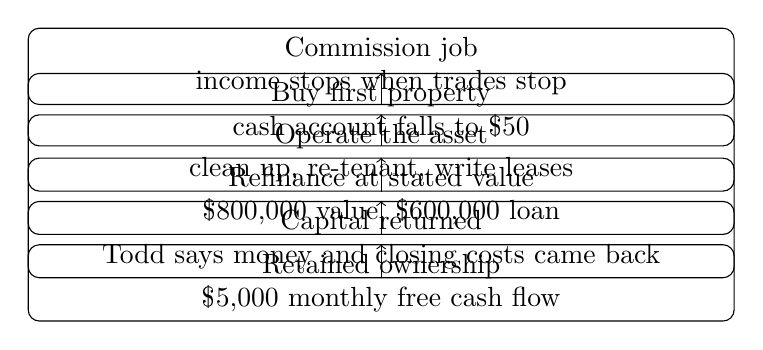
\begin{tikzpicture}[
  box/.style={draw, rounded corners, align=center, text width=0.72\linewidth, minimum height=0.62cm},
  node distance=0.55cm
]
\node[box] (job) {Commission job\\income stops when trades stop};
\node[box, below of=job] (buy) {Buy first property\\cash account falls to \$50};
\node[box, below of=buy] (work) {Operate the asset\\clean up, re-tenant, write leases};
\node[box, below of=work] (refi) {Refinance at stated value\\\$800,000 value, \$600,000 loan};
\node[box, below of=refi] (return) {Capital returned\\Todd says money and closing costs came back};
\node[box, below of=return] (cash) {Retained ownership\\\$5,000 monthly free cash flow};
\draw[->] (job) -- (buy);
\draw[->] (buy) -- (work);
\draw[->] (work) -- (refi);
\draw[->] (refi) -- (return);
\draw[->] (return) -- (cash);
\end{tikzpicture}
\caption{The first-property capital cycle, reconstructed from the transcript rather than from a validated board figure.}
\end{figure}

\subsection{Question \& Answer}

\paragraph{Question.}
How can a deal return the capital and still produce cash flow?

\paragraph{Answer.}
In Todd's telling, the answer is not magic leverage; it is the sequence. First he controls the property. Then he changes its operation by improving the tenant situation and the physical condition. The property is then refinanced at a higher value. The new loan returns the original capital and closing costs, while the property remains under ownership and produces monthly free cash flow.

The arithmetic we can safely show is limited:
\begin{align}
\Delta V
&=
V_{\mathrm{refi}}-P_{\mathrm{buy}} \\
&=
\$800{,}000-\$575{,}000 \\
&=
\$225{,}000,
\end{align}
and the implied equity after the refinance, using only the stated value and loan, is
\begin{equation}
E_{\mathrm{after\ refi}}
=
V_{\mathrm{refi}}-L_{\mathrm{refi}}
=
\$800{,}000-\$600{,}000
=
\$200{,}000.
\end{equation}

These are not complete profit calculations. We do not know renovation cost, exact closing costs, prior debt structure, tax consequences, or financing terms. The safe point is structural: operating improvement made a refinance possible, and the refinance changed trapped capital into returned capital plus continuing ownership.

\section{Books, Time Horizons, and One Property}

After the intense first-property story, the interview slows down. The host asks about the book that changed Todd's business life. Todd names Tony Robbins, especially the lesson that people overestimate what they can do in one year and underestimate what they can do in five. He then widens the point into reading generally: a book condenses decades of experience into a form that can be absorbed quickly.

That claim connects naturally to Todd's own book on commercial real estate. The book becomes a bridge from personal story to durable rules. His first takeaway is that wealthy people in many industries own real estate. His second is that property type must fit the owner's life. His third is that commercial property is more possible than beginners think, especially if the first property is one the owner can manage directly.

The strongest retirement claim is deliberately simple: buy one property, pay it off over twenty to twenty-five years, and it can become a source of retirement support. We should preserve the claim as Todd's interview advice rather than inflate it into a universal financial theorem. The implied mechanism is long-horizon ownership:
\begin{equation}
\text{property control}
\longrightarrow
\text{debt paydown}
\longrightarrow
\text{owned asset}
\longrightarrow
\text{retirement cash-flow potential}.
\end{equation}

The lecture's rhythm here is important. Todd does not jump from the first deal to a giant portfolio. He pauses at the smallest durable unit: one property that fits the owner and can be understood.

\section{The Capital Obstacle: The Deal Is Harder Than the Money}

The host then raises the objection that many beginners feel immediately: do you need a lot of money to buy real estate? Todd's answer is the most compressed maxim in the interview: go find a deal.

His example is deliberately extreme. He points to Aventura Mall nearby and estimates, roughly, that it might be worth \$3 billion. Then he asks us to imagine that someone offers it for \$1 billion, but requires closing the next morning. His claim is that capital could be found because the deal would be so compelling.

We can write the illustrative arithmetic, with the caveat that the \$3 billion number is Todd's rough estimate and the \$1 billion price is hypothetical:
\begin{align}
V_{\mathrm{mall,guess}}&\approx \$3\mathrm{B},\\
P_{\mathrm{hypothetical}}&=\$1\mathrm{B},\\
\frac{P_{\mathrm{hypothetical}}}{V_{\mathrm{mall,guess}}}
&=
\frac{1}{3}
\approx 33.3\%.
\end{align}

The implied discount, in this hypothetical, is
\begin{equation}
1-\frac{1}{3}
=
\frac{2}{3}
\approx 66.7\%.
\end{equation}

This is not an appraisal and not a real offer. It is a teaching device. Todd is separating two problems:
\begin{itemize}
\item finding a deal that makes economic sense;
\item finding capital for a deal that already makes economic sense.
\end{itemize}

\subsection{Question \& Answer}

\paragraph{Question.}
If a beginner has no money and no credit, why does Todd say the deal is the hard part?

\paragraph{Answer.}
Because in Todd's model, capital is attracted to asymmetry. If the property can be bought at a price far below a credible value, and if the buyer can explain the opportunity clearly, then investors with capital have a reason to participate. The beginner's scarce contribution is not necessarily the check. It may be the discovery, analysis, and presentation of a good deal.

This does not remove risk. It changes the task. The first job is no longer ``be rich enough to buy property outright.'' The first job is to learn a market well enough to recognize and bring forward a deal that capital wants.

\section{Operating Edge: Local Control and In-House Work}

Once the capital obstacle is answered, the host asks how Todd's company stands out in a competitive industry. Todd's answer is operational, not glamorous. The firm keeps its properties within roughly 250 to 300 miles, close enough that he can drive to a property, understand what is going on, handle the issue, and return home.

Let
\begin{equation}
R_{\mathrm{properties}}\approx 250\text{--}300\ \mathrm{miles}.
\end{equation}
This radius is not just a geography fact. It is an operating constraint. It defines the area inside which local knowledge, tenant relationships, property management, leasing, and accounting can remain integrated.

Todd also says the leasing team, accounting team, and property management team are in-house. The reason is control. One property manager knows what another manager is doing. A tenant in one property may refer a tenant for a vacancy in another. The advantage is not merely ownership of buildings; it is ownership of the operating information around the buildings.

\begin{figure}
\centering
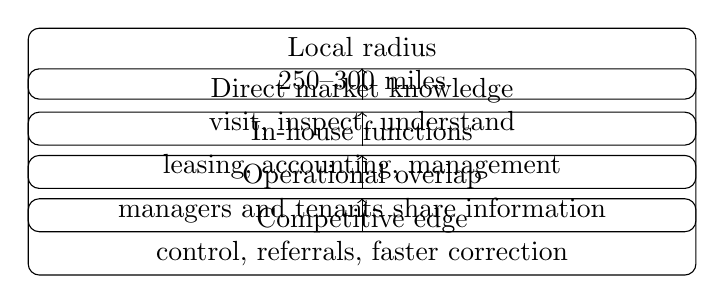
\begin{tikzpicture}[
  box/.style={draw, rounded corners, align=center, text width=0.68\linewidth, minimum height=0.62cm},
  node distance=0.55cm
]
\node[box] (radius) {Local radius\\250--300 miles};
\node[box, below of=radius] (knowledge) {Direct market knowledge\\visit, inspect, understand};
\node[box, below of=knowledge] (teams) {In-house functions\\leasing, accounting, management};
\node[box, below of=teams] (overlap) {Operational overlap\\managers and tenants share information};
\node[box, below of=overlap] (edge) {Competitive edge\\control, referrals, faster correction};
\draw[->] (radius) -- (knowledge);
\draw[->] (knowledge) -- (teams);
\draw[->] (teams) -- (overlap);
\draw[->] (overlap) -- (edge);
\end{tikzpicture}
\caption{Todd's operating edge, reconstructed from his description of local ownership and in-house teams.}
\end{figure}

This is where the first-property story scales. The first deal required direct action: cleaning, re-tenanting, writing leases. The company version of that same logic is an in-house machine for noticing problems, leasing space, collecting information, and maintaining control.

\section{Scale, Contrarian Timing, and the Reason to Keep Going}

The biggest deal Todd discusses was closed the previous December: a \$25 million acquisition of shopping-center property that had never been on the market. He describes a father and son building the centers decades earlier, over roughly a ten-year span, before ownership passed down through heirs and became complicated. The asset contained 165,000 square feet.

The raw facts are:
\begin{equation}
P_{\mathrm{large\ deal}}=\$25\mathrm{M},
\qquad
A=165{,}000\ \mathrm{sq\ ft}.
\end{equation}
A simple descriptive metric is the purchase price per square foot:
\begin{equation}
\frac{\$25{,}000{,}000}{165{,}000}
\approx
\$151.52/\mathrm{sq\ ft}.
\end{equation}
This number should not be over-read. We are not given occupancy, rents, cap rate, debt terms, tenant quality, or property condition. It is useful only as a scale marker.

The next question asks about investment advice. Todd's answer is contrarian: go against the grain. If everyone is afraid, that may be the moment to look harder. If everyone is aggressively buying the same thing, that may be the moment to become cautious. He gives examples from office, retail, industrial, and multifamily, but the underlying rule is broader:
\begin{equation}
\text{herd enthusiasm} \Rightarrow \text{raise caution},
\qquad
\text{excessive fear} \Rightarrow \text{search for mispriced deals}.
\end{equation}

The final movement of the interview turns from money to motive. Todd says that becoming wealthy requires knowing why one wants wealth. The wrong why is display: cars, dinners, image. The better why is financial freedom, family security, helping parents, sending children to college, and sleeping without fear of next month's bills.

Then comes the reset question: if the bank account went to zero, what would remain? Todd's answer is that money is not the only capital. Knowledge, contacts, bank relationships, reputation, and domain love remain. In a compact form:
\begin{equation}
\text{rebuildable capital}
=
\text{skill}
+
\text{contacts}
+
\text{bank relationships}
+
\text{reputation}
+
\text{domain commitment}.
\end{equation}

That is why the chapter ends where it began, but at a deeper level. The first story was about cash going to almost zero. The final story is about what survives even if cash goes to zero again.

\section{Summary}

The interview's main mechanism is the first-property cycle: acquire control, improve operations, refinance against a higher value, recover capital, and keep cash flow. The numerical spine is modest but concrete: \$575,000 purchase price, \$800,000 refinance value, \$600,000 loan, 75\% inferred loan-to-value, and \$5,000 monthly free cash flow.

Around that mechanism Todd builds a larger doctrine. Mentorship matters when advice becomes action. Wealth is not the same as visible consumption. One property can matter if the owner understands it and holds it through time. Capital may chase a good enough deal, but the deal must be found first. Scale comes from operating control: local properties, in-house teams, tenant knowledge, and repeatable management. Finally, the most durable form of wealth is not a number by itself, but the ability to rebuild: judgment, relationships, reputation, and a field one is willing to return to.